% =====================================================================
%  2026-04-21 — 第一次去光華:今華電子採購記
% =====================================================================

\subsection*{今日目標}

\begin{itemize}[leftmargin=2em,itemsep=0pt]
  \item 帶著 4/19 跟 Gemini 對話整理出來的「必買 / 可以等 / 實驗室借用」三張清單,
        到光華商場地下室實地採買,把麵包板實驗的零件補齊。
  \item 走「無烙鐵」路線:這次只湊到能在麵包板上插出類比前端 TIA 的東西,
        STM32 排針焊接、SFH 2440、烙鐵都留給網購。
  \item 用 Gemini chat 當「邊走邊問的店內顧問」,遇到老闆指著我看不懂的東西、
        或是貨架上 MCP6002 缺貨時即時備援。
\end{itemize}

\subsection*{地點 \& 時間}

\textbf{今華電子有限公司台北分公司}(北市新生南路一段 12 巷 2 號,TEL: 02-23921111),
2026-04-21 (一) 13:41 結帳。光華地下室,離源達科技不遠。

\subsection*{邊買邊問:Gemini 在現場救了哪些急?}

實際逛貨架時,清單上的東西不是每樣都長得跟想像中一樣,
這時候用手機拍照丟給 Gemini 確認非常有用。今天用上的幾個臨場提問:

\begin{itemize}[leftmargin=2em,itemsep=0pt]
  \item \textbf{「這個可以當作 TM1637 嗎?」} —— 包裝寫「4 位數時鐘顯示模組」
        沒寫 TM1637,Gemini 教我隔著塑膠袋找 \texttt{VCC/GND/DIO/CLK} 四根排針,
        確認就是同一顆。OK,放進籃子。
  \item \textbf{「\(\,\)EIC-1104 / 1106 / 1108 哪一塊比較適合?」} —— 老闆櫃台同時擺了三個尺寸。
        Gemini 推 1104:雙區設計可做「類比區 / 數位區」分離,1106/1108 太大佔桌面,
        對螢幕貼近量測反而不方便。
  \item \textbf{「\(\,\)EIC-1104 還需要 MB102 嗎?」} —— EIC-1104 帶接線柱,看起來像高級電源板,
        但其實它只是「馬路」,不會自己發電。沒實驗室的大電供時,必買 MB102 給 5 V 轉 3.3 V。
  \item \textbf{「BPW34 又會叫什麼名字?」} —— 怕老闆聽不懂型號,Gemini 教我退而求其次叫
        「光敏二極體」、「平頭的接收管」、或「矽光電池」。實際上今華有原裝 Vishay BPW34,
        所以這招沒用上,但學起來。
  \item \textbf{「\(\,\)Pico PR2040 可以嗎?」} —— 我把 RP2040 跟 Pico 搞混,Gemini 解釋
        RP2040 就是 Pico 上面那顆晶片;Pico 板就是 RP2040 + 周邊。我要的是那塊板。
  \item \textbf{「沒有 MCP6002 還有哪些放大器可以選擇呢?」} —— **這是今天最痛的一題**。
        架上沒 MCP6002,Gemini 提了 LMC6482、MCP6022、TLC2272 三個 DIP-8 替代品,
        又警告 LM358 / TL072 / NE5532 是地雷不能拿。最後\textbf{今天店裡這幾顆都沒有貨},
        op-amp 空手而回(詳見下面「漏買」一節)。
  \item \textbf{「那 MCP6008 可以嗎?」} —— 看貨架瞄到一個型號像的 IC,問了 Gemini 才知道
        MCP6008 根本不存在;我可能跟 MCP3008 (那是 8 通道 ADC) 或 MCP608 搞混。差點買錯。
  \item \textbf{「DC 圓頭哪一根是正極?」} —— 拿到「9V 電池扣轉 DC 公頭」轉接頭,兩根金屬針沒標示。
        Gemini 教我用三用電表蜂鳴檔測導通,找出哪根通到中心、哪根通到外圈,然後遵循 MB102 的
        「\textbf{內正外負}」(Center Positive)規範。
\end{itemize}

\subsection*{購買清單與收據}

最後刷掉 \(\textbf{TWD 1{,}530}\) 現金,收據如圖~\ref{fig:0421-receipt}。

\begin{figure}[H]
  \centering
  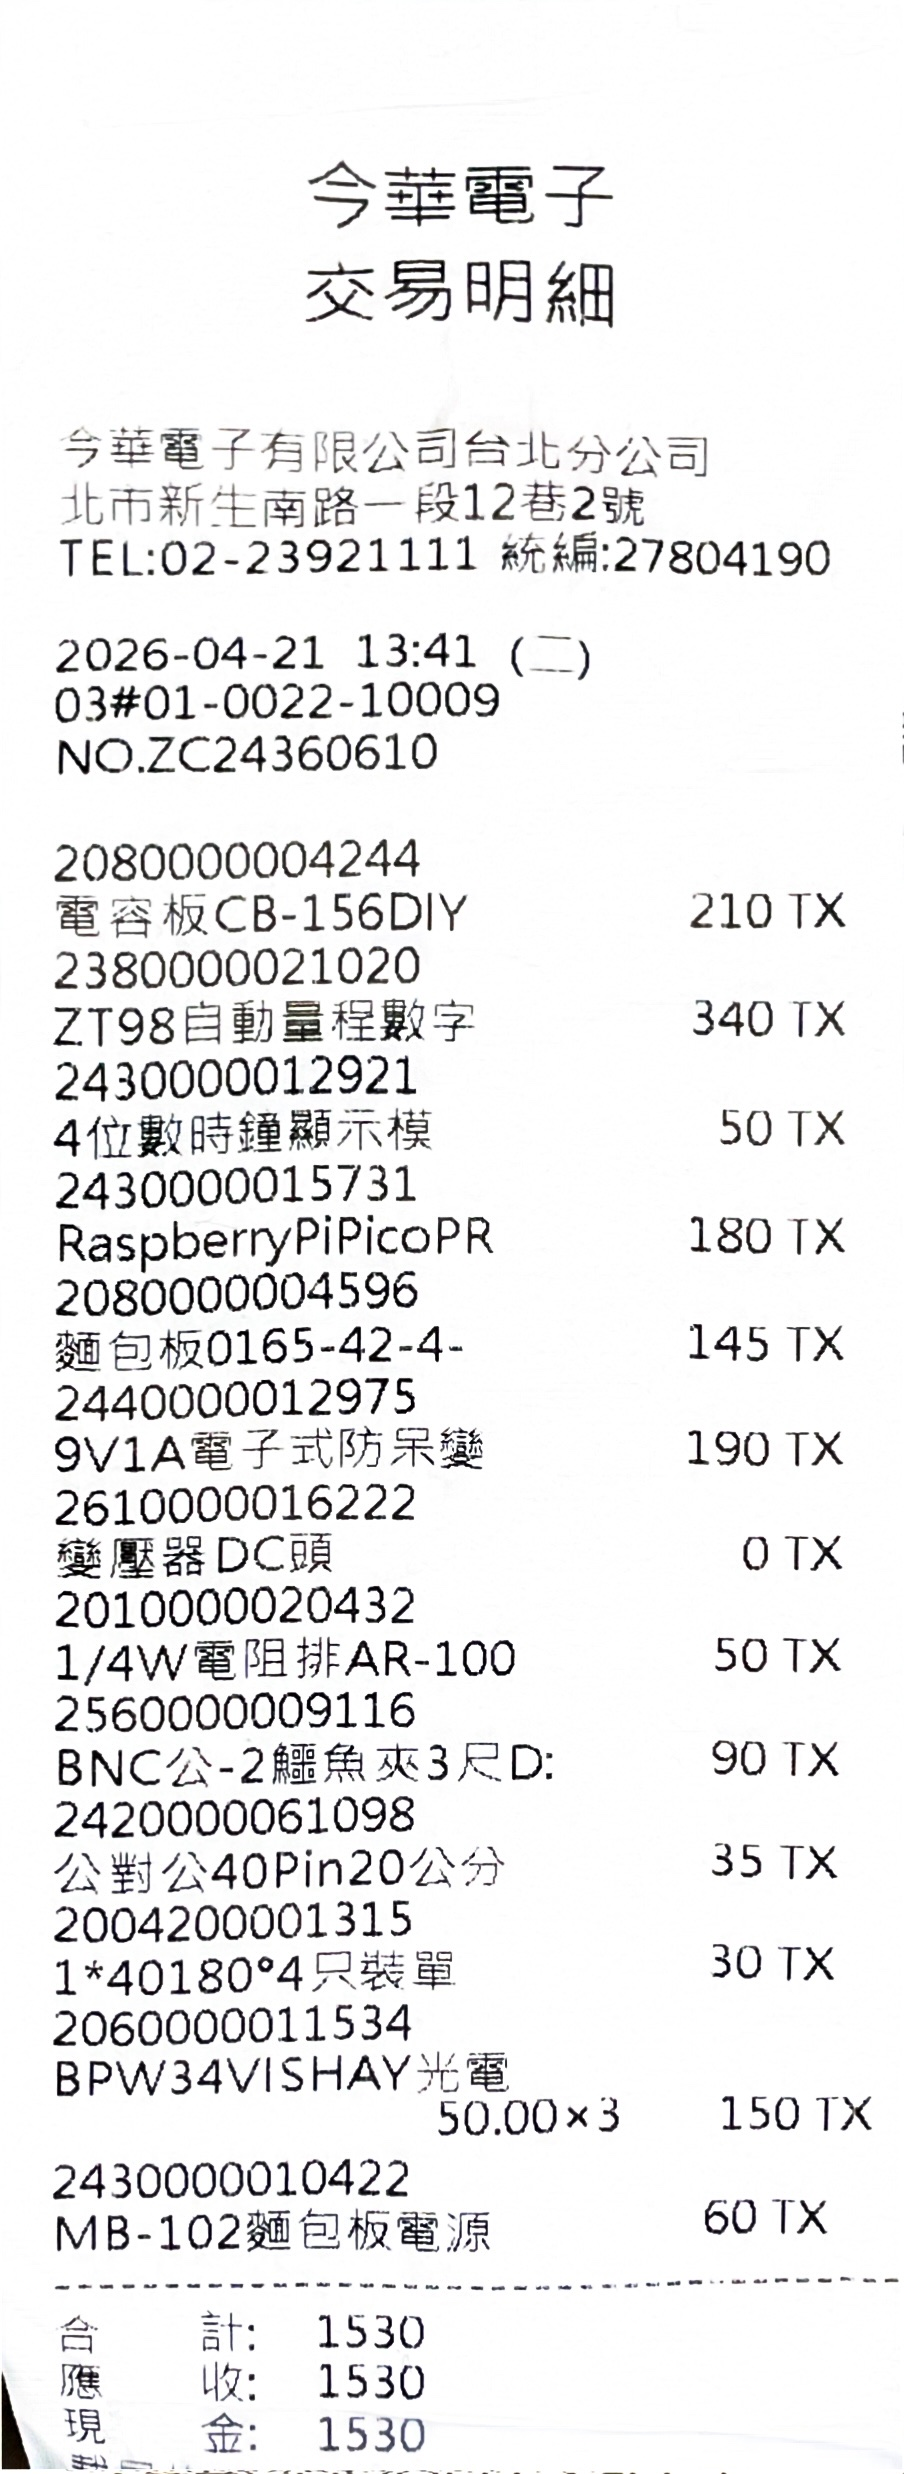
\includegraphics[width=0.55\linewidth]{2026-04-21/今華電子交易明細0421.jpg}
  \caption{今華電子 2026-04-21 13:41 交易明細,合計 TWD 1530。}
  \label{fig:0421-receipt}
\end{figure}

明細整理:

\begin{table}[H]
  \centering
  \caption{4/21 今華電子採購明細。}
  \label{tab:0421-bom}
  \begin{tabular}{llrr}
    \toprule
    類別 & 品項 & 數量 & 小計 (TWD) \\
    \midrule
    儀器 & ZT98 自動量程數位三用電表          & 1 & 340 \\
    平台 & EIC-1104 等級麵包板 (型號 0165-42-4-)  & 1 & 145 \\
    電源 & MB-102 麵包板電源模組               & 1 & 60  \\
    電源 & 9V / 1A 電子式防呆變壓器             & 1 & 190 \\
    電源 & 變壓器 DC 頭(9V 電池扣轉接)         & 1 & 0   \\
    MCU  & Raspberry Pi Pico (RP2040, Type-C 版) & 1 & 180 \\
    顯示 & TM1637 4 位 7 段顯示模組             & 1 & 50  \\
    感測 & Vishay BPW34 光電二極體              & 3 & 150 \\
    被動 & 電容板 CB-156 DIY 電容組合包         & 1 & 210 \\
    被動 & 1/4 W 色碼電阻排 AR-100              & 1 & 50  \\
    接線 & 公對公 40-pin 20 cm 杜邦線            & 1 & 35  \\
    接線 & 1$\times$40 180° 單排排針(4 入裝)    & 1 & 30  \\
    量測 & BNC 公頭轉 2 鱷魚夾線,3 ft            & 1 & 90  \\
    \midrule
    \multicolumn{3}{r}{\textbf{合計(現金)}} & \textbf{1{,}530} \\
    \bottomrule
  \end{tabular}
\end{table}

幾個現場決定的細節:

\begin{itemize}[leftmargin=2em,itemsep=0pt]
  \item \textbf{BPW34 買 3 顆}是備援 —— 第一次接 TIA 很容易接反極性或燒掉,150 元便宜保險。
  \item \textbf{電容板 CB-156 DIY} 是臨時加碼。Gemini 原本只要求 10 pF、22 pF、104 各幾顆,
        但老闆推這盒 156 種規格全包,210 元划算,以後不會缺電容值,
        後面要調補償電容也比較有彈性。
  \item \textbf{9V/1A 變壓器 + DC 頭}是 Gemini 提醒的「容易忽略的致命細節」:
        MB-102 的圓孔必須吃 7--12 V 輸入,USB 5 V 不夠。沒這條線今天就白跑了。
  \item \textbf{BNC--鱷魚夾線 90 元}是預先為後續實驗室示波器架設準備的;
        系上實驗室通常只給 BNC 介面,沒這條線連不上麵包板。
\end{itemize}

\subsection*{走到源達補貨:MCP6004 \(\times\,\)2}

今華結帳後,因為 op-amp 整批缺貨,直接走去隔壁的\textbf{源達科技}補。源達櫃台
剛好有 \textbf{MCP6004}(DIP-14,內含 4 顆 op-amp),雖然 Gemini 提醒 MCP6004
是「14 根腳的大蜈蚣、未用的 op-amp 要接成 voltage follower 否則高頻干擾」,
但內部規格跟 MCP6002 一模一樣,接腳 100\% 相容專題需求,當下就拿了。

\textbf{兩顆 MCP6004,單價忘記了,暫記每顆 50,合計 100 TWD(等發票補齊)}。
這樣專題靈魂的類比核心元件總算到手,類比前端 TIA 接下來就可以開工。

\subsection*{今天還沒買的東西(留給網購)}

\begin{itemize}[leftmargin=2em,itemsep=0pt]
  \item \textbf{波段開關(增益旋鈕)\& 撥動開關(AC/DC 模式)} —— 今華有貨但決定暫緩。
        Gemini 提醒過機械波段開關接腳粗,直插麵包板會撐壞簧片;
        先用「手動拔線換 \(R_F\)」模擬切檔就好,等真的進外殼再買。
  \item \textbf{烙鐵 / 焊錫 / SFH 2440 / SMD 轉 DIP 轉接板 / 3.7 V LiPo / TP4056 / LDO} ——
        全列為「可以等(網購)」,今天不買。
\end{itemize}

\subsection*{今日實驗進度}

回家拆完戰利品,只跑到「電源軌通電」這一步就收工:

\begin{enumerate}[leftmargin=2em,itemsep=2pt]
  \item 把 9 V/1 A 變壓器跟 DC 公頭轉接頭組裝起來。先用三用電表蜂鳴檔確認轉接頭中心極對應的金屬針,
        把變壓器的線接到中心極 (+),外圈那根接外圈 (-)。
  \item 上電前最後 double check:三用電表轉到 DC V,紅探針進中心孔、黑探針碰外圈,
        讀到 \textbf{+9.0 V},極性沒接反。
  \item 把轉接頭插進 MB-102 的 5.5$\times$2.1 mm 圓孔,MB-102 上的小撥桿撥到 3.3 V 檔位。
  \item 把 MB-102 跨插到 EIC-1104 麵包板的電源軌上。
  \item 用三用電表量麵包板紅軌跟藍軌之間的電壓,讀到 \textbf{\(\sim\)3.30 V 直流},
        電源軌通電成功。
\end{enumerate}

\textbf{今天就停在這。}沒接 op-amp、沒接 PD、沒進 TIA 階段 —— 因為今華沒 op-amp 的時候我已經
逛累了,源達補完 MCP6004 拿回家天已經黑;先把電源接通、確認沒短路冒煙,
等明天再開始照 Gemini 給的步驟接 TIA。

\subsection*{今日心得}

\begin{itemize}[leftmargin=2em,itemsep=0pt]
  \item 第一次去光華,最大收穫不是材料,而是學會\textbf{「邊走邊問」的工作流}:
        把 Gemini 當駐店顧問,拍照確認模組、問替代品、問封裝差異 ——
        現場決策品質會高很多。
  \item 跟老闆對話得用對術語:\textbf{DIP-8 vs SMD}、\textbf{Rail-to-Rail}、
        \textbf{1P3T / 1P4T},講清楚對方才不會推錯貨。聽到「LM358 雙電源音響款很好用」
        要會回「不行,單 3.3 V 軌會被削掉」。
  \item \textbf{單一店家不可靠}:今華缺 op-amp 時所幸隔壁源達有 MCP6004,
        以後關鍵元件應該事先打電話問 / 列備援店家清單,別假設一家就湊得齊。
  \item 第一天回家只敢做「上電不冒煙」這一步,看似沒進度,
        但其實\textbf{把電源軌驗到 3.30 V}本身就是後面所有實驗的前提 ——
        TIA 接錯燒 op-amp 大半時候是電源段就有問題,先把這層基底確定,
        後續除錯空間才會小。
  \item 接下來:1) 把 MCP6004 接上麵包板做 voltage follower 試一次 (Gemini 教的安全測試法),
        確認晶片活著;2) 接 TIA 並掛 BPW34 量光;3) 下單 SFH 2440 + 轉接板;
        4) 下單 Pinecil / PTS200 智慧烙鐵;5) Pico 排針等烙鐵到再焊。
\end{itemize}
